%!TEX root = ./HW2.tex

\section{100 Cities}
\subsection{Results}
For 100 cities, the best solution is MCTS.  EA performs similarly, but has a larger standard deviation.  As the space grows, the more directed search of MCTS might be able to better the space than the large sampling that EA and SA do.  In such a large space, the somewhat random search that EA and SA carry out make it hard to ever stumble upon the best solution.


\begin{table}[H]
\centering
\begin{tabular}{|c|c|c|c|c|c|}
\hline
Algorithm               & \begin{tabular}[c]{@{}c@{}}Total Solutions\\ Generated\end{tabular} & \begin{tabular}[c]{@{}c@{}}Average Min\\ Distance\end{tabular} & St Dev & \begin{tabular}[c]{@{}c@{}}Average\\ Run Time (s)\end{tabular} & St Dev  \\ \hline
Simulated Annealing     & 10,000                                                              & 13,796                                                         & 1,742  & 3.70e-6                                                        & 8.94e-7 \\ \hline
Evolutionary Algorithm  & 10,000                                                              & 12,222                                                         & 1,337  & 9.89                                                           & 0.03    \\ \hline
Monte Carlo Tree Search & 10,000                                                              & 12,047                                                         & 937    & 3.70                                                           & 0.15    \\ \hline
\end{tabular}
\caption{Comparison of Solution Quality and Run Time for Each Method with 100 Cities}
\label{tab:25Comparison}
\end{table}

% insert image of example solutions found by search

\begin{figure}[H]
	\centering
    \begin{minipage}{0.45\textwidth}
        \centering
        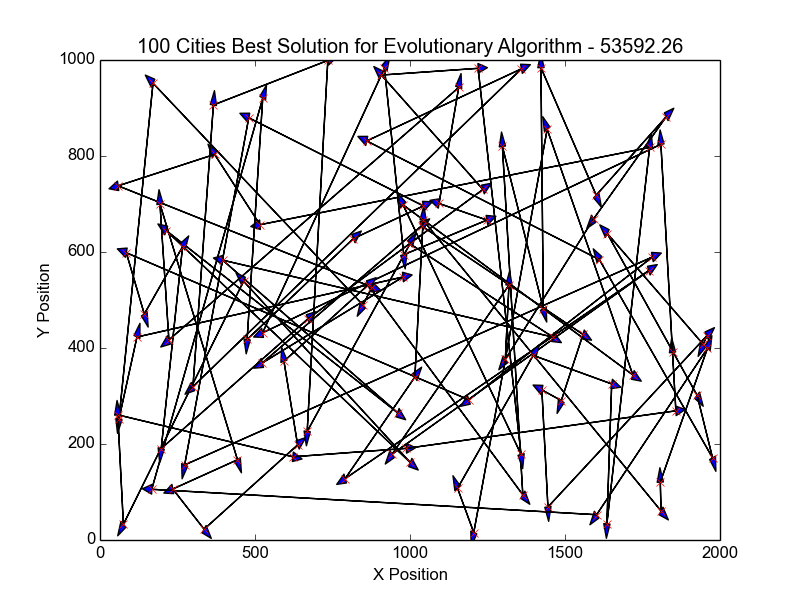
\includegraphics[width=0.9\textwidth]{100City_EA.png} % first figure itself
        \caption{Best Solution for 100 Cities with Evolutionary Algorithm}
        \label{fig:100city_EA}
    \end{minipage}\hfill
    \begin{minipage}{0.45\textwidth}
        \centering
        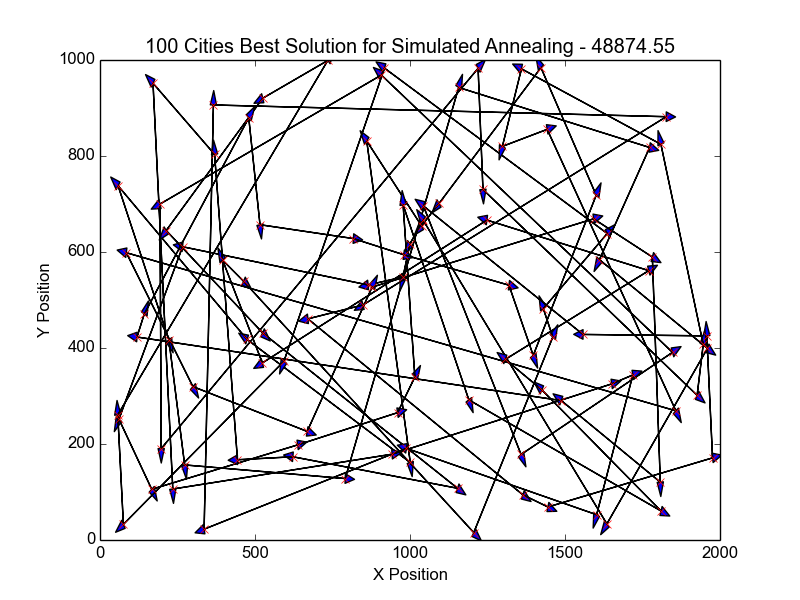
\includegraphics[width=0.9\textwidth]{100City_SA.png} % second figure itself
        \caption{Best Solution for 100 Cities with Simulated Annealing}
        \label{fig:100city_SA}
    \end{minipage}\hfill
    \begin{minipage}{0.45\textwidth}
        \centering
        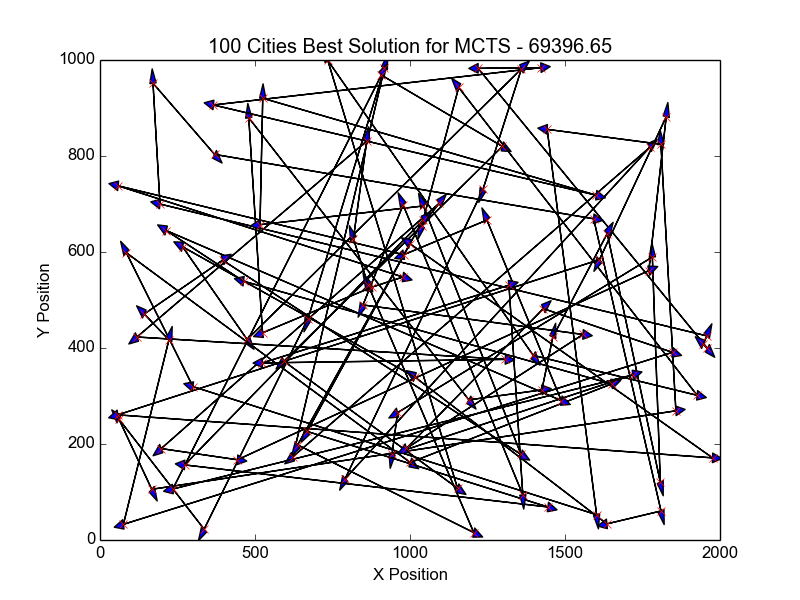
\includegraphics[width=0.9\textwidth]{100City_MCTS.png} % third figure itself
        \caption{Best Solution for 100 Cities with MCTS}
        \label{fig:100city_MCTS}
    \end{minipage}\hfill
    \begin{minipage}{0.45\textwidth}
		\centering
		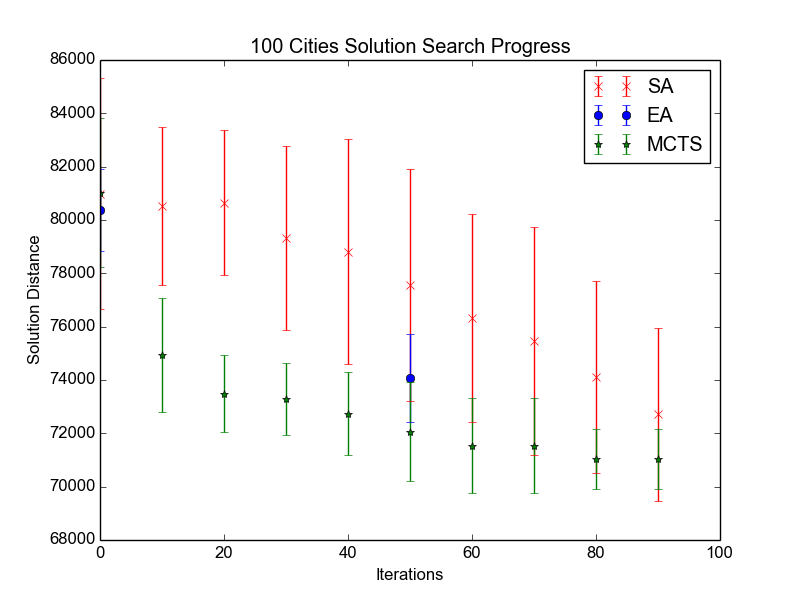
\includegraphics[width=0.9\textwidth]{100City_Solutions.png}
		\caption{Solution Progression for 100 Cities}
		\label{fig:100city_Solution}
    \end{minipage}\hfill
\end{figure}

